\documentclass[12pt]{article}
\usepackage[utf8]{inputenc}
\usepackage{upquote}
\usepackage[margin=1in]{geometry} 
\usepackage{amsmath,amsthm,amssymb}
\usepackage{graphicx}
\usepackage{listings}
\newenvironment{statement}[2][Statement]{\begin{trivlist}
\item[\hskip \labelsep {\bfseries #1}\hskip \labelsep {\bfseries #2.}]}{\end{trivlist}}
\usepackage{xcolor}
\usepackage{booktabs}
\usepackage{xcolor}
\usepackage{subfigure}



\title{Handin 1}

\begin{document}
\maketitle

\section{Introduction}

In this project we develop a testing protocol and performance metric for algorithms provided in common optimization toolboxes. The algorithm we test on includes the Ellipsoid function(f1), the Rosenbrock Banana Function(f2), the Log-Ellipsoid Function(f3), the Attractive-Sector Function(f4), and the Sum of Different Powers Function(f5). We focus on three different optimization algorithms, including the Broyden-Fletcher-Goldfarb-Shanno(BFGS), Newton-CG, and trust-region.

Our metrics reflects the the four criteria for good algorithms. For \textbf{Robustness}, we develop test on different initial guesses and dims of the initial guesses. For \textbf{Accuracy} we record the precision when the optimizer reaches the tolerance rate. We also run with multiple initial guesses and calculate the running time in average, in order to prove the \textbf{Stability} and \textbf{Resource Efficiency}. % TODO cite NO notes 
Also we plot the convergence process with the 2-norm distance in log scale to see the algorithm performance in visual. 

%Outlines the report.
%Contains information about contents, (research) questions and overall structure.

\section{Theory}

%Your Theoretical contributions.
%Theoretical considerations that shape choices in the experimental section.
Here we are going to introduce our theoretical considerations that shape the choices of initial guesses in the experimental section.

We narrow down some theoretical convergence status of the given functions by calculating Gradient and Hessian, and find the minimiser using the second order sufficient conditions.

The gradient of a function is a vector of its first-order partial derivatives. A point $x^*$ is a critical point if the gradient is zero, and the critical points are candidates for local minima points.

\begin{equation}
\nabla f(x^*) = 0
\label{critical}
\end{equation}

The Hessian H(x) is a matrix of second-order partial derivatives of f(x). It provides information about the curvature of the function at a given point. It provides information about the curvature of the function at a given point.

To determine if a critical point $x^*$ is a local minimizer, we mainly apply the Second Order Sufficient Conditions, which includes the the $H(x^*)$ is positive definite (all eigenvalues are positive), then $x^*$ is a strict local minimizer by equation~\ref{critical}.


%The optimizers in scipy package aim to find the local minimum value of a function starting from a given array, namely initial guess(x0). % TODO reference to scipy official document: https://docs.scipy.org/doc/scipy/reference/generated/scipy.optimize.minimize.html

%The BFGS is a quasi-Newton method for unconstrained optimization, approximating the Hessian matrix to find a local minimum. It is gradient-based, so results depend on the initial guess and may converge to different local minima. % TODO reference



\section{Experiments}

%Description of the experiments performed.
%Description of procedure and evaluation metrics.
%Also includes choices of parameters

We choose different values and dims of initial guess, alpha and optimizers to find the minimum value among the five functions. We record the average runtime of different initial guess(x0), error rate when reaching the tolerance point and success rate. The variables are listed in Table. % TODO add table  

\begin{table}[h!]
\label{table:rule}
\centering
\begin{tabular}{cc}
\toprule
 \textbf{Item} & \textbf{Value} \\ 
\midrule
\textbf{x0 Sample Num} & 5 \\
\textbf{x0 Dim} & {2,5,10} \\
\textbf{x0 Distribution} & Normal with random seed = 42 \\
\textbf{Alpha(in f1)} & {10,100,1000} \\
\textbf{Max Iterations} & 1000 \\
\textbf{Epsilon on Tolerance} & 1e-10 \\
\bottomrule
\end{tabular}
\caption{Variants for experiment setups; x0 means the initial guess}
\end{table}

We plot the convergence process with the 2-norm distance in log scale to see the algorithm performance in visual. The log scale is applied to reveal the difference when the values of different optimizer functions got closer on a very small scale.

\section{Results and Discussion}

For the various testing functions, we are going to discussion them separately in the following sections. The log-scale convergence graph is shown in Figure~\ref{fig:convgraph}.

\begin{figure}[ht]
\centering
\subfigure[]{
    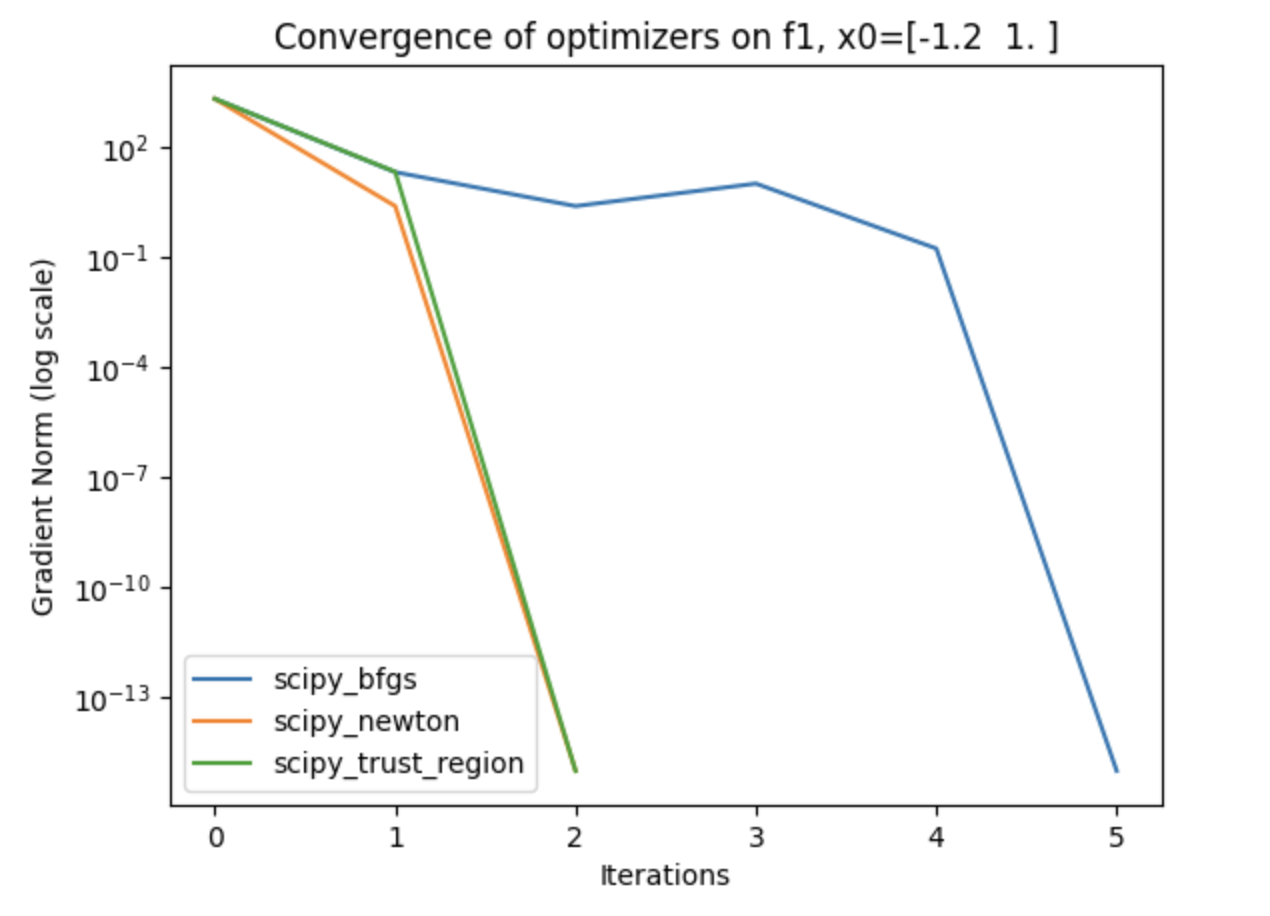
\includegraphics[width=0.25\columnwidth, keepaspectratio]{pics/f1-d2}
\label{fig:f1}
}
\subfigure[]{
    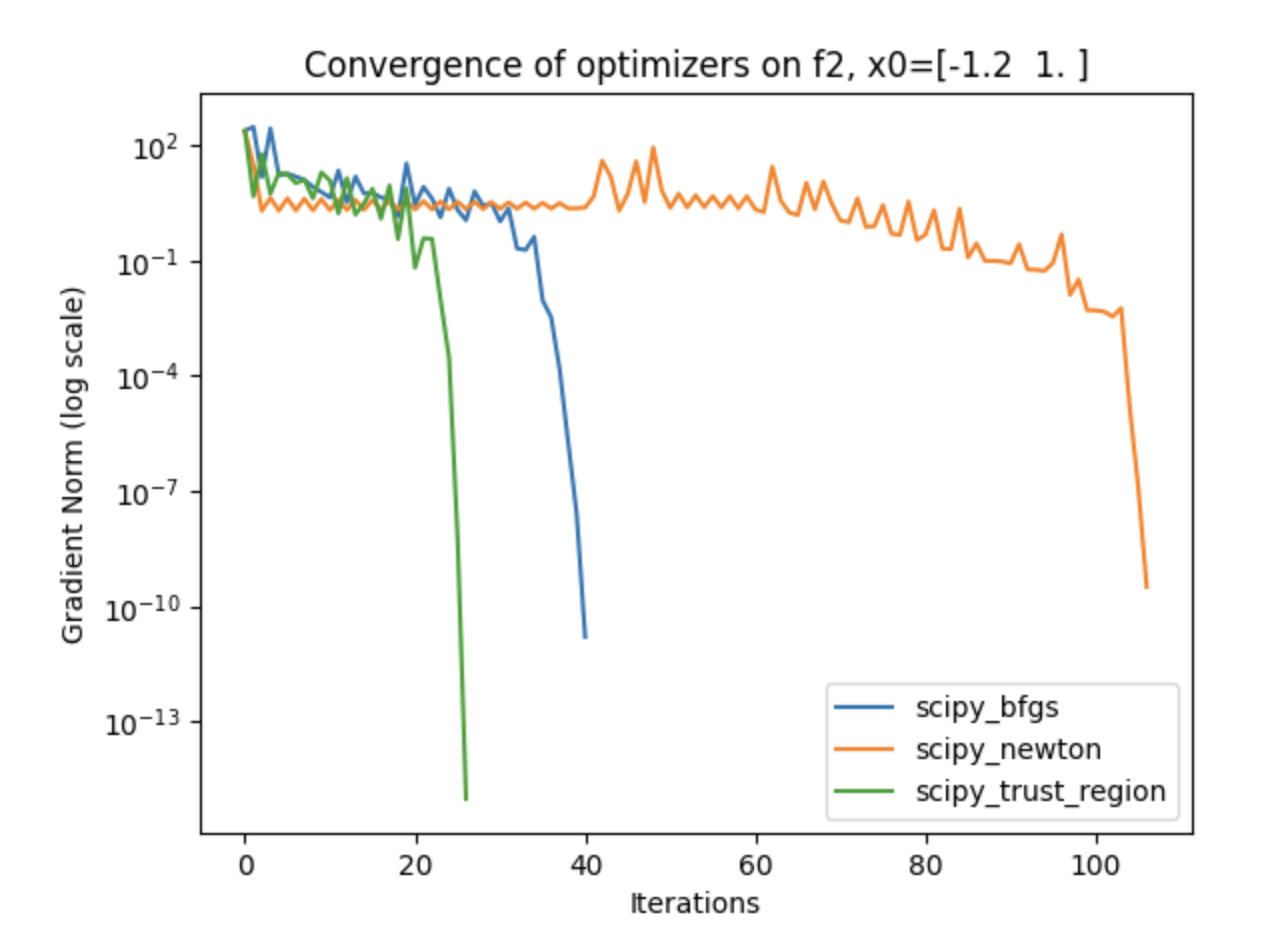
\includegraphics[width=0.25\columnwidth, keepaspectratio]{pics/f2-d2}
    \label{fig:f2}
}
\subfigure[]{
    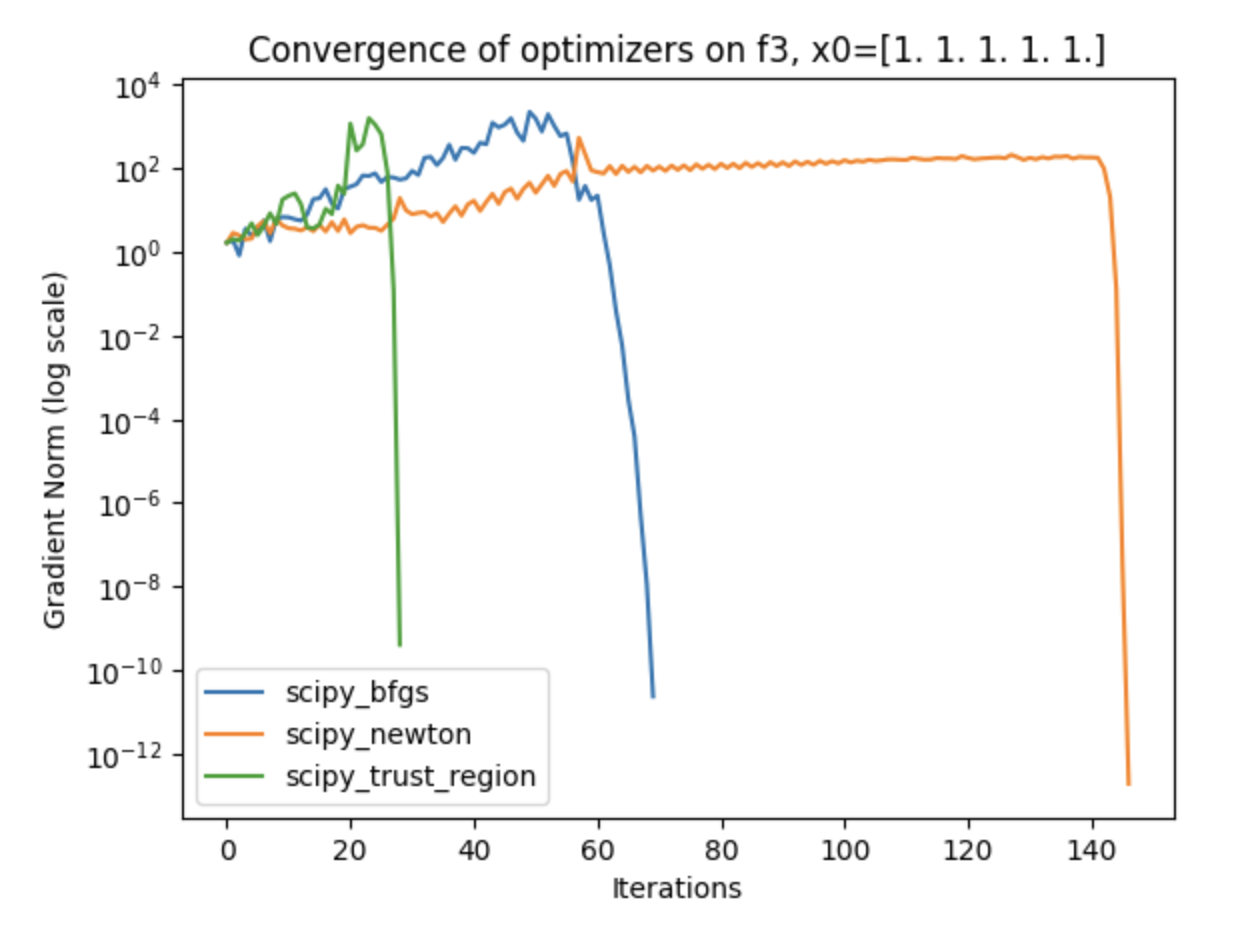
\includegraphics[width=0.25\columnwidth, keepaspectratio]{pics/f3-d5}
    \label{fig:f3}
}
\subfigure[]{
    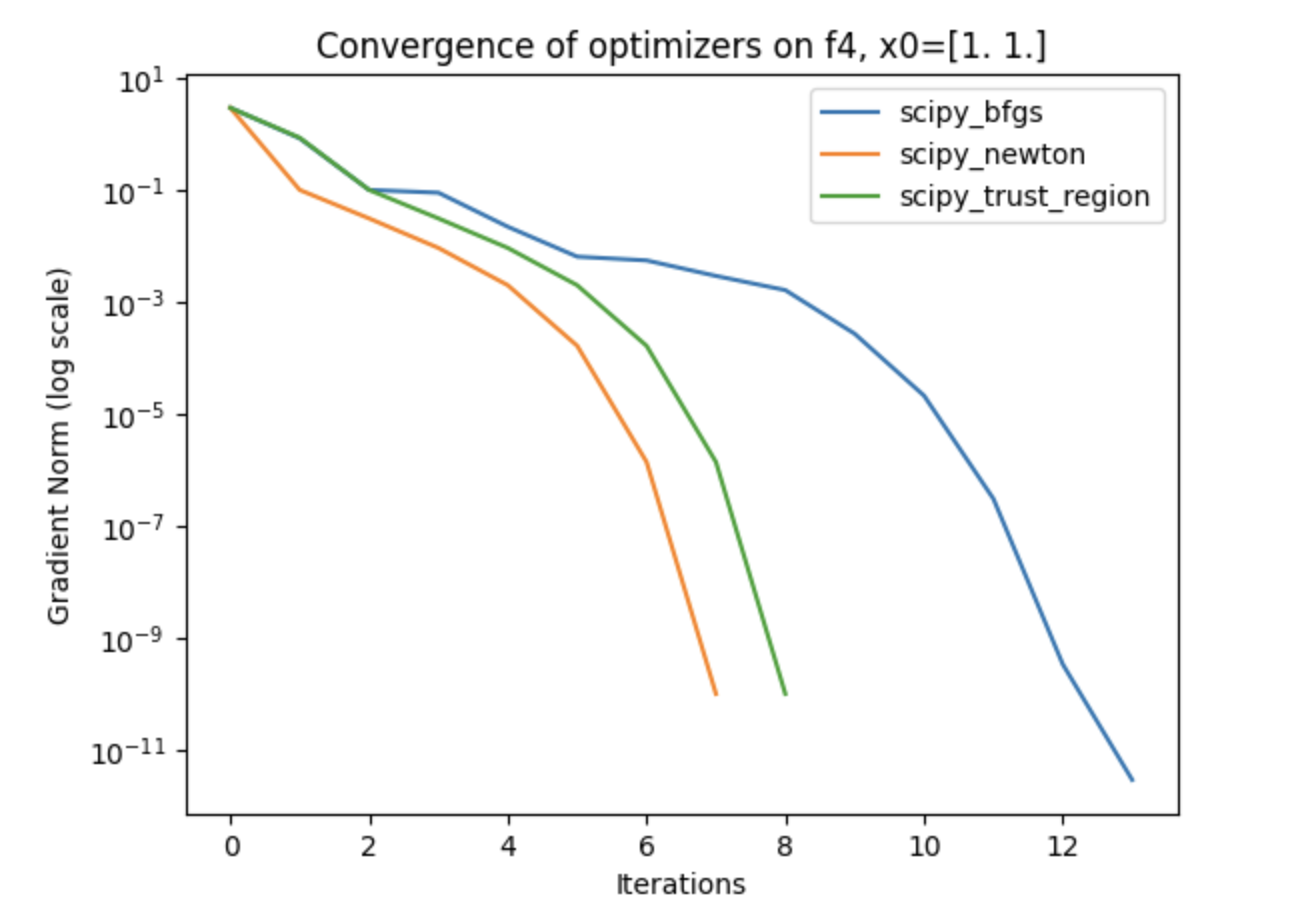
\includegraphics[width=0.25\columnwidth, keepaspectratio]{pics/f4-d2}
    \label{fig:f4}
}
\subfigure[]{
    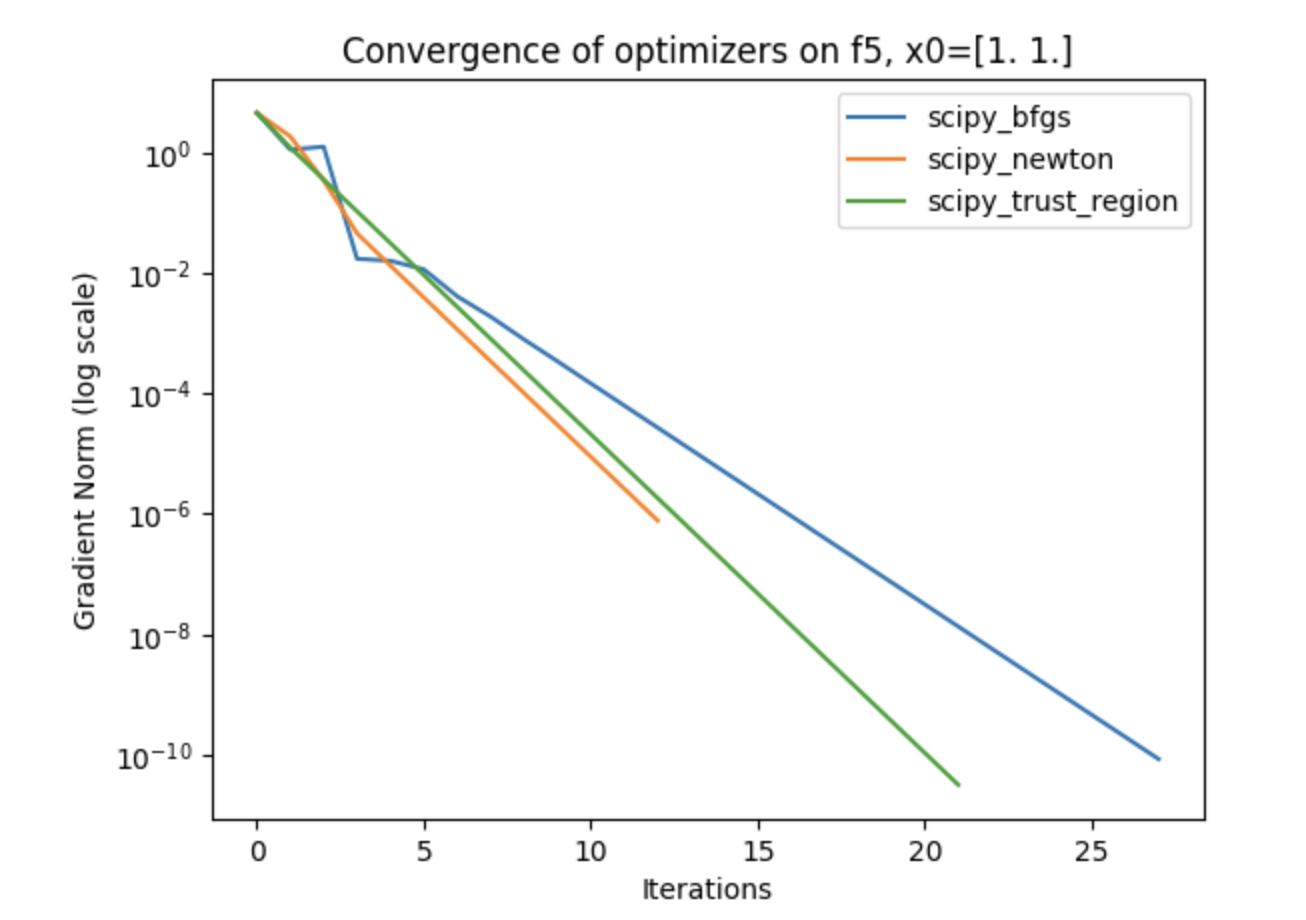
\includegraphics[width=0.25\columnwidth, keepaspectratio]{pics/f5-d2}
    \label{fig:f5}
}
\caption[]{Convergence graph(log scale) of the three optimize algorithms on the five functions, analyzing iterations}
\label{fig:convgraph}
\end{figure}

\subsection{The Ellipsoid Function(f1)}

\subsubsection{Speed and Accuarcy}
As issued in Figure~\ref{fig:f1}, for the fixed initial guessing point $x_0=(-1.2,1.0)$, both the three algorithms succeed in converging the optimal solution, with final gradient norm $\approx1e-15$. Trust-Region demonstrated the best efficiency in both runtime and function evaluations, while BFGS achieved the highest precision. According to the testing protocol, our test result is in Table~\ref{tab:f1}, and our discussion is as follow.

\textbf{Evaluation Iterations} 
Newton-CG and Trust-Region outperforms BFGS on the number of evaluation iterations takes to convergence, with 3 against 6. This suggests that second-order methods (Newton and trust-region) adapted more efficiently to the problem’s curvature than the quasi-Newton approach (BFGS).

\textbf{Runtime}
Trust-Region achieved the fastest runtime (0.001253s), followed by Newton-CG (0.002091s) and BFGS (0.002473s). 

\textbf{Precision}
BFGS attained the smallest distance to the optimum (2.71e-20), and both Newton-CG and Trust-Region reached comparable solutions with a slightly larger final distance ($\approx2.22e-16$).

\begin{table}[h]
    \centering
\begin{tabular}{lccc}
    \toprule
    Metric & scipy\_bfgs & scipy\_newton & scipy\_trust\_region \\
    \midrule
    Final Solution Point & $[0, 2.71\times10^{-20}]$ & $[2.22\times10^{-16}, 2.17\times10^{-19}]$ & $[-2.22\times10^{-16}, 0]$ \\
    Distance to Optimum & $2.71\times10^{-20}$ & $2.22\times10^{-16}$ & $2.22\times10^{-16}$ \\
    Function Evaluations & 6 & 3 & 3 \\
    Final Function Value & $7.35\times10^{-37}$ & $4.94\times10^{-32}$ & $4.93\times10^{-32}$ \\
    Final Gradient Norm & $1.00\times10^{-15}$ & $1.00\times10^{-15}$ & $1.00\times10^{-15}$ \\
    Convergence Success & True & True & True \\
    Runtime (s) & 0.002473 & 0.002091 & 0.001253 \\
    \bottomrule
\end{tabular}
    \caption{Optimization results for the Ellipsoid Function.}
    \label{tab:f1}
\end{table}

\subsubsection{Different Initial Guesses and Optimizer Choices}
We also explore the different dims and alpha value and their influence on the speed of convergence, measured by iterations. For all the three optimizers running on f1, the higher the dim is, the larger the iterations takes to reach tolerance will be. The Trust-Region has a relevant small iteration number, even if the alpha is larger(as 1000).


\subsection{The Rosenbrock Banana Function(f2)}

As shown in Figure~\ref{fig:f2}, for the fixed initial point $x_0=(-1.2,1.0)$, all three algorithms successfully converged to the optimal solution, with final gradient norms close to (1e-15). Trust-Region exhibited the best efficiency in both runtime and function evaluations, while BFGS achieved the highest precision.  According to Table~\ref{tab:f2}, we have the following discussion:

\textbf{Evaluation Iterations}  
Trust-Region required the fewest function evaluations ($27$), outperforming BFGS ($41$) and Newton-CG ($107$). This suggests that second-order methods generally adapted more efficiently to the problem’s curvature, but Newton-CG struggled due to the function's high condition number of its Hessian matrix.

\textbf{Runtime}  
Trust-Region achieved the fastest runtime ($0.004087s$), followed by BFGS ($0.007580s$) and Newton-CG ($0.009386s$), further confirming its efficiency.  

\textbf{Precision}  
Trust-Region reached the exact optimum with zero error. BFGS achieved a final distance of $(1.23e-12)$, while Newton-CG had a slightly larger error of $(8.12e-10)$, indicating slower convergence to high precision.

\begin{table}[h]
    \centering
\begin{tabular}{lccc}
    \toprule
    Metric & scipy\_bfgs & scipy\_newton & scipy\_trust\_region \\
    \midrule
    Final Solution Point & $[1, 1]$ & $[1, 1]$ & $[1, 1]$ \\
    Distance to Optimum & $1.24\times10^{-12}$ & $8.12\times10^{-10}$ & $0.00$ \\
    Function Evaluations & 41 & 107 & 27 \\
    Final Function Value & $4.35\times10^{-25}$ & $1.32\times10^{-19}$ & $0.00$ \\
    Final Gradient Norm & $1.62\times10^{-11}$ & $3.24\times10^{-10}$ & $1.00\times10^{-15}$ \\
    Convergence Success & True & True & True \\
    Runtime (s) & 0.00758 & 0.009386 & 0.004087 \\
    \bottomrule
\end{tabular}
    \caption{Optimization results for the Rosenbrock Banana Function.}
    \label{tab:f2}
\end{table}

\subsection{The Log-Ellipsoid Function(f3))}

\subsection{The Attractive-Sector Function(f4)}

\subsection{The Sum of Different Powers Function(f5)}


%Presentation of the outcome of the experiments.
%Discussion of the results, including the knowledge gained from the theoretical questions.
%Also contains discussion of experimental shortcomings.

\section{Conclusion}

%What knowledge have we gained?
%Could we answer the question we set out to answer in the Introduction?


\end{document}
